\chapter{Logica a pass transistor}

Ora vogliamo trovare una logica che abbia i vantaggi del CMOS e la semplicità dell'nMOS. Una possibile soluzione è la logica a pass transistor.

\paragraph{}
Fino ad ora i segnali in ingresso viene usato per attivare il transistor ed è quest'ultimo che  sposta l'uscita, dunque il segnale in ingresso non agisce direttamente sull'uscita ma ha azione indiretta.

In questa logica il segnale di ingresso viene usato anche per pilotare l'uscita, dunque l'ingresso non è più solo collegato al gate del transistore bensì è anche collegato al source e drain.

\paragraph{}

Quando il gate	è a	1,	il segnale in	ingresso al	source	del	
transistore passa in	uscita. Si	può effettuare una notevole riduzione nel numero dei
transistor.

\paragraph{Porta AND}


\begin{itemize}
    \item Quando B	=	0,	è abilitato solo	il pass inferiore e	l'uscita è 0
    \item Quando B	=	1,	in	uscita si trova A
\end{itemize}

\begin{figure}[htbp]
    \centering
    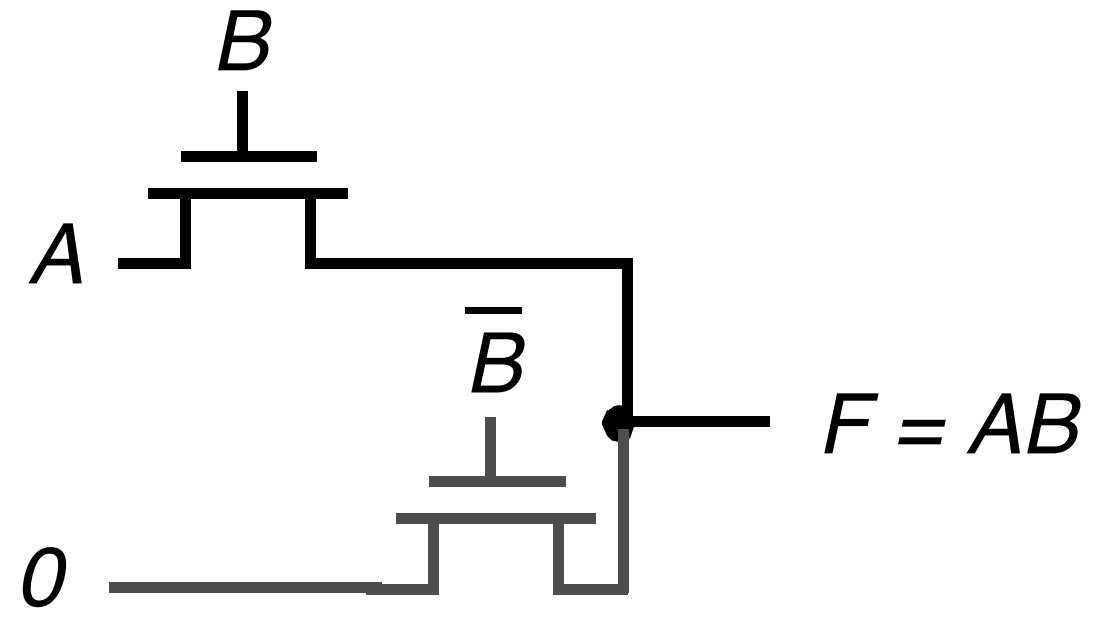
\includegraphics[width=0.35\linewidth]{img/and_pass.png}
    
    
\end{figure}


In logica CMOS sono 6 i transistor da utilizzare al posto di 4 come in questo caso (2 in figura e 2 per B'), vi è un notevole risparmio!

\section{Livelli dei segnali}

Come	visto per	l'inverter con	carico a	saturazione,	il
transistore nMOS non	è in	grado di	caricare l'uscita fino a $V_{DD}$.

\begin{itemize}
    \item L'uscita arriva al	più a	$V_{DD} - V_{TN}$ perché poi	il canale svanisce;
    \item La	situazione,	come	visto,	è peggiorata dall'effetto body,	visto che $V_{SB}$ non	è nulla
    \item Nel caso dell'inverter,	si arrivava a	1.55	V (2.5 - 0.6 - effetto body)	invece di	2.5	V
\end{itemize}

\newpage
\begin{figure}[htbp]
    \centering
    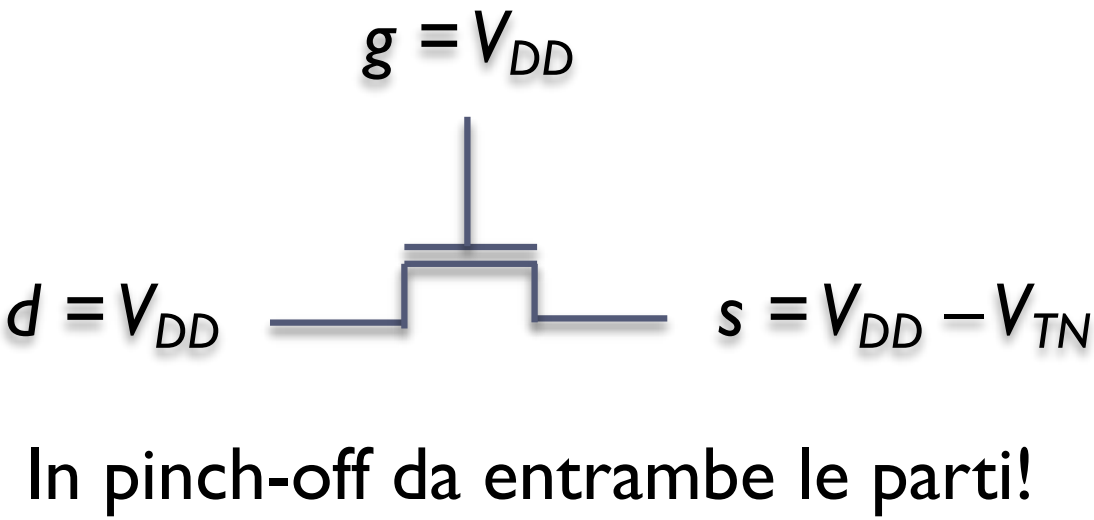
\includegraphics[width=0.35\linewidth]{img/imgggg.png}
\end{figure}

\paragraph{}
Dunque conduce bene solo uno dei due valori. Possiamo usare transistori nMOS o pMOS, degradano	il	segnale	a	causa	della	tensione	di	soglia	in	 maniera	complementare.


\begin{figure}[htbp]
    \centering
    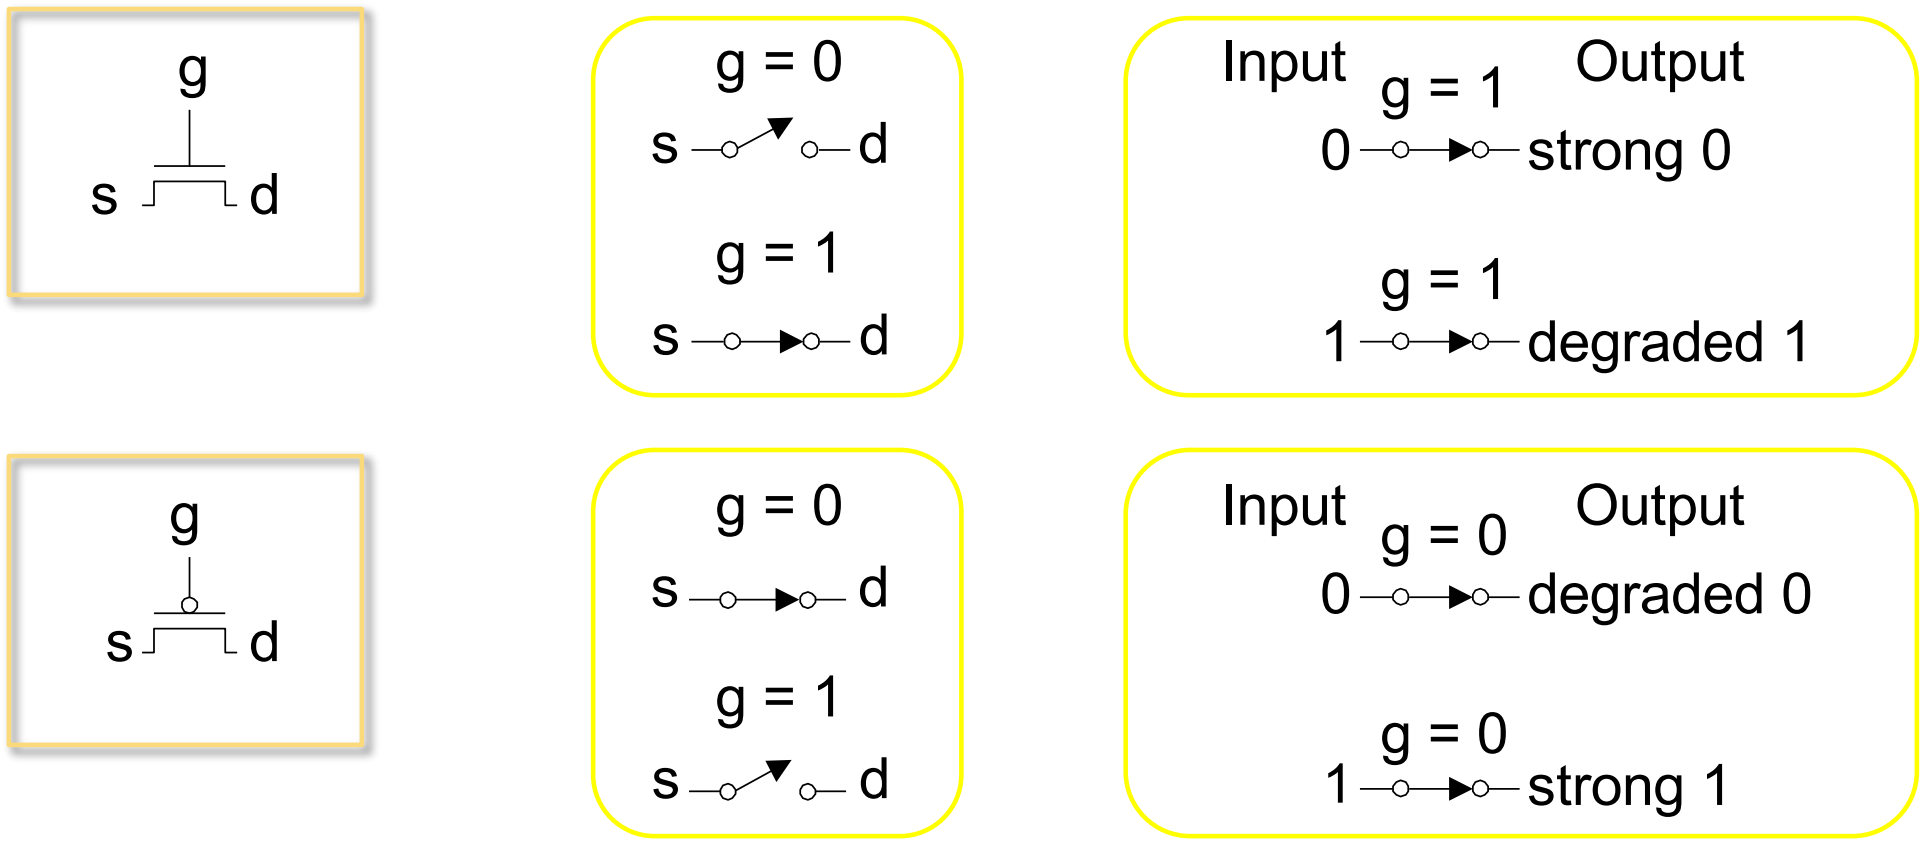
\includegraphics[width=0.7\linewidth]{img/npmos.png}
    
    
\end{figure}


\newpage
\section{Transmission gate}
Un idea è quella di metterli in parallelo, i transmission	gate	sono	coppie	complementari, fanno passare bene entrambi i livello.

\paragraph{}

Vi è un problema: \textbf{non restoring} il	rumore	di	ingresso	viene	passato	sull'uscita. In logica CMOS questo non avviene, il segnale viene ripulito.

\begin{figure}[htbp]
    \centering
    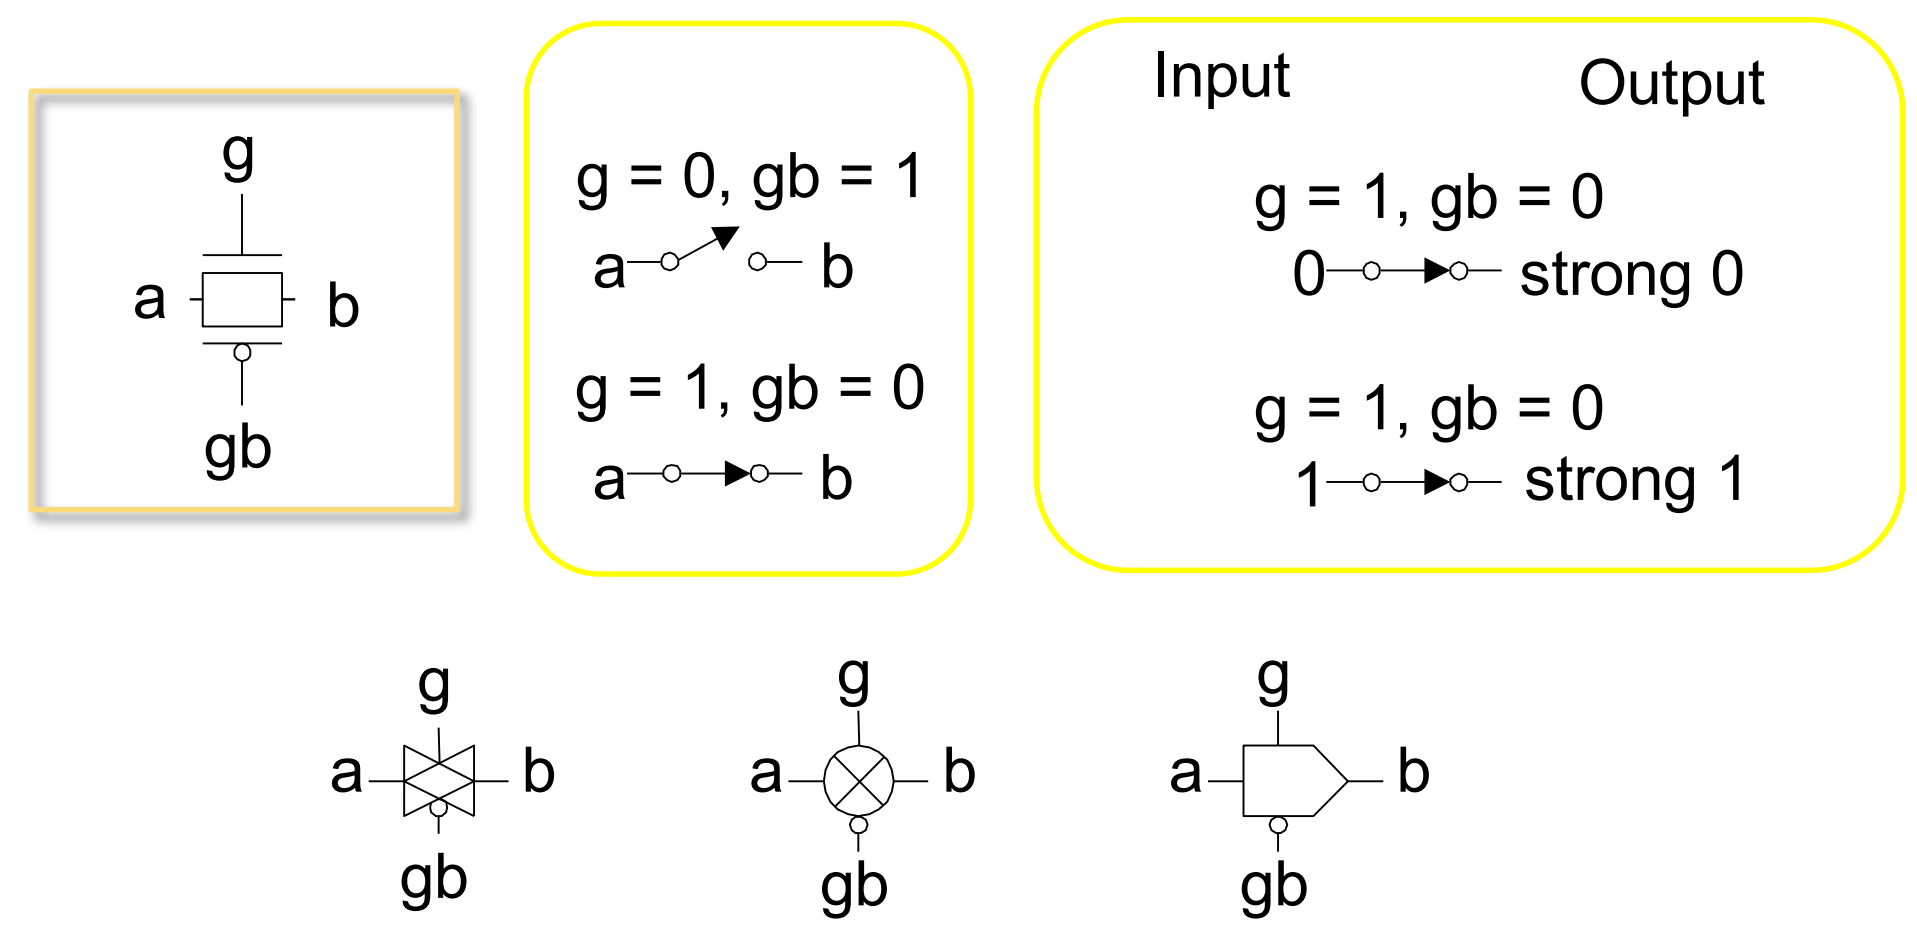
\includegraphics[width=0.6\linewidth]{img/trans_gatre.png}   
    
\end{figure}

Questo meccanismo spreca un transistore in più, e notare che serve anche il complemento.


\paragraph{Si	realizzi	la	funzione	f =	as +	bs'}

\paragraph{}
In	CMOS	occorrono	20	transistori	(14	soluzione	con	NAND). Con	transmission	gate	ne	bastano	6.

\begin{figure}[htbp]
    \centering
    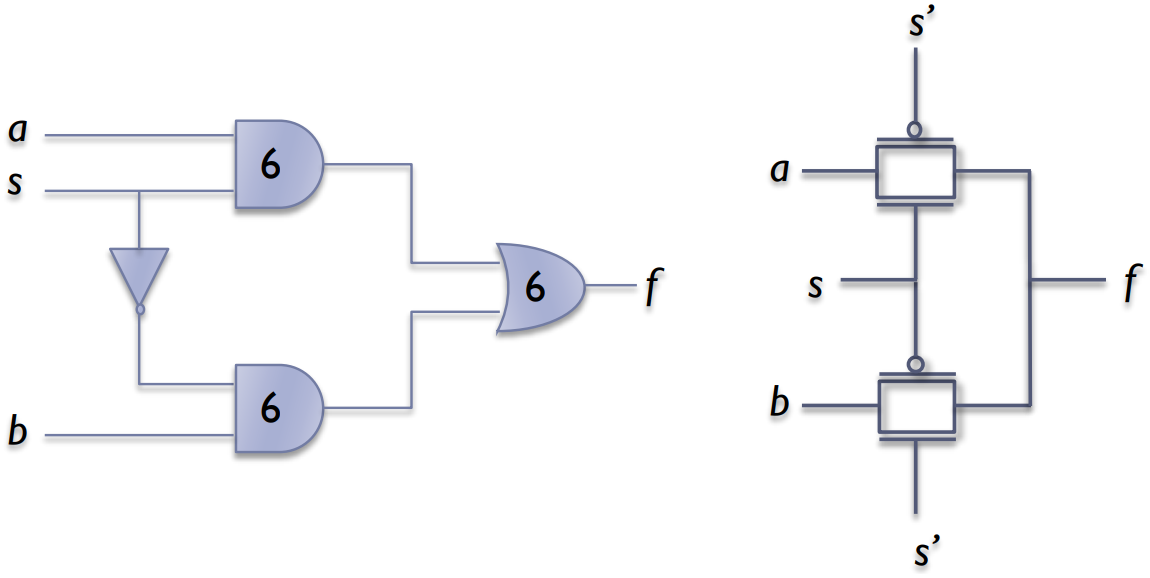
\includegraphics[width=0.7\linewidth]{img/aksdcjvubc.png}        
\end{figure}

\newpage
\section{Funzione che usa la logica transmission gate}

Data F = AB + A'C' + AB'C

% \begin{figure}[htbp]
%     \centering
%     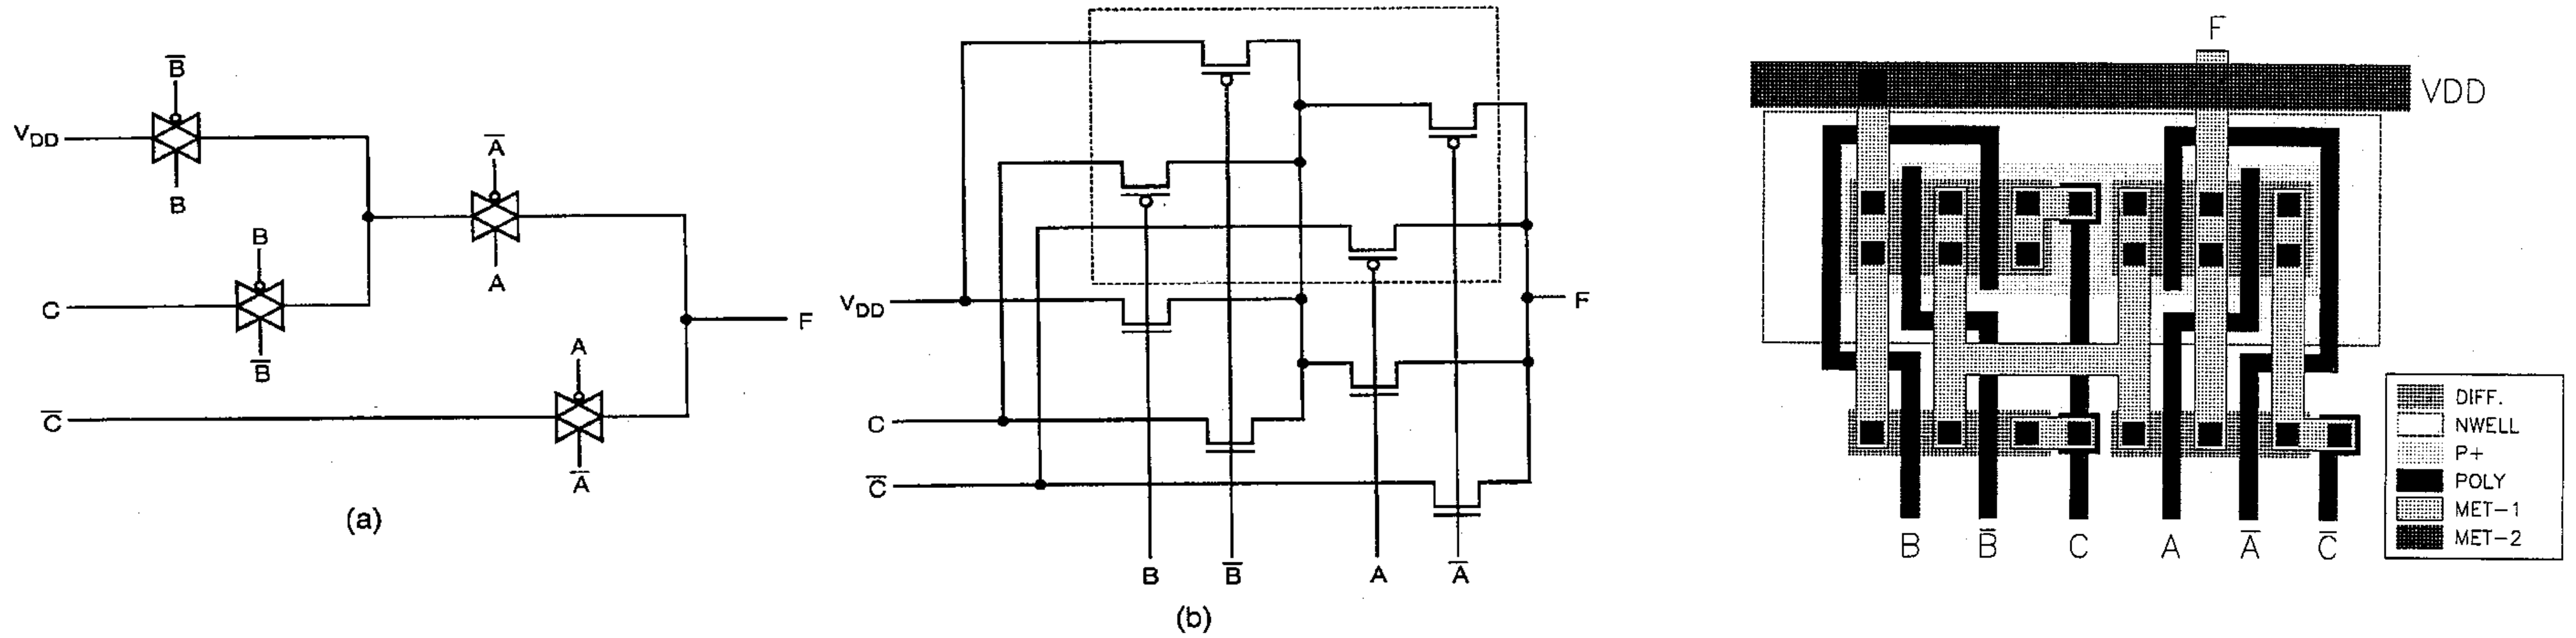
\includegraphics[width=1\linewidth]{img/funzione_pass.png}    
    
% \end{figure}
\begin{figure}[htbp]
    \centering
    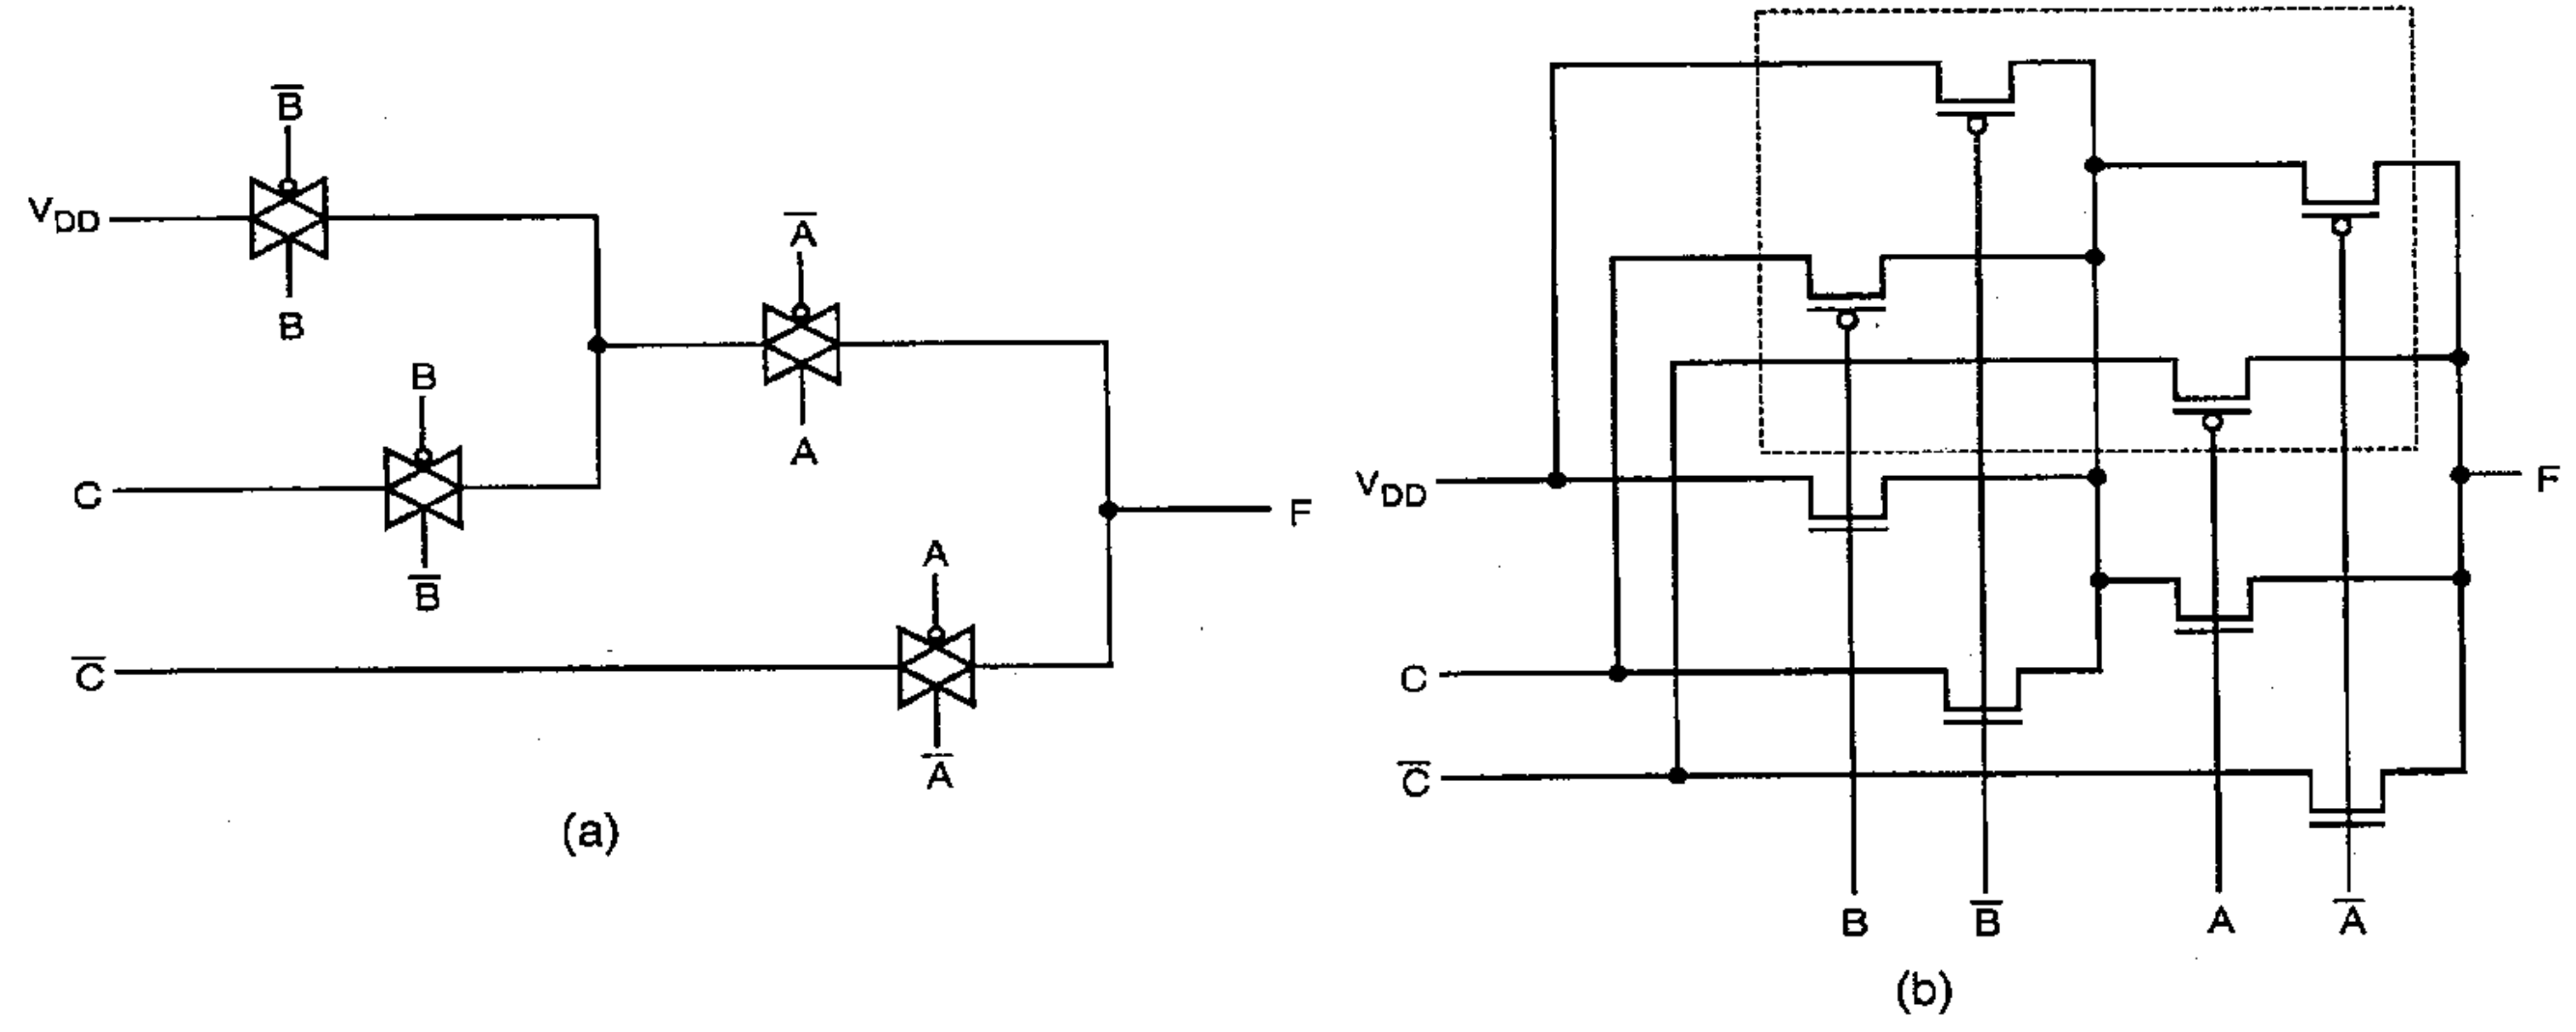
\includegraphics[width=0.7\linewidth]{img/trans_circ_integrato.png}
    
    
\end{figure}

Funzione di 3 variabili realizzata tramite
transmission gate (a), 14 transistori inclusi gli invertitori contro 34 per realizzazione CMOS.

Layout ottimizzato raggruppando i transistori
p ed n assieme (b), richiede un solo n-well.


% \begin{figure}[htbp]
%     \centering
%     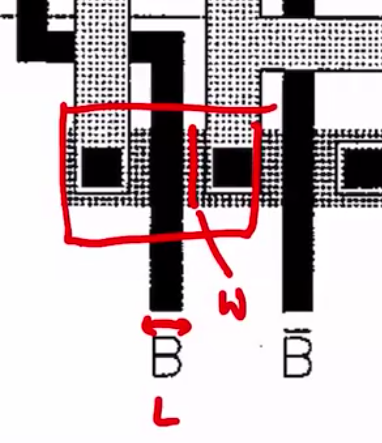
\includegraphics[width=0.2\linewidth]{img/transistore_circ_integrato.png}   
%     \caption{Il tranistore in un circuito integrato}
% \end{figure}


\begin{figure}[htbp]
    \centering
    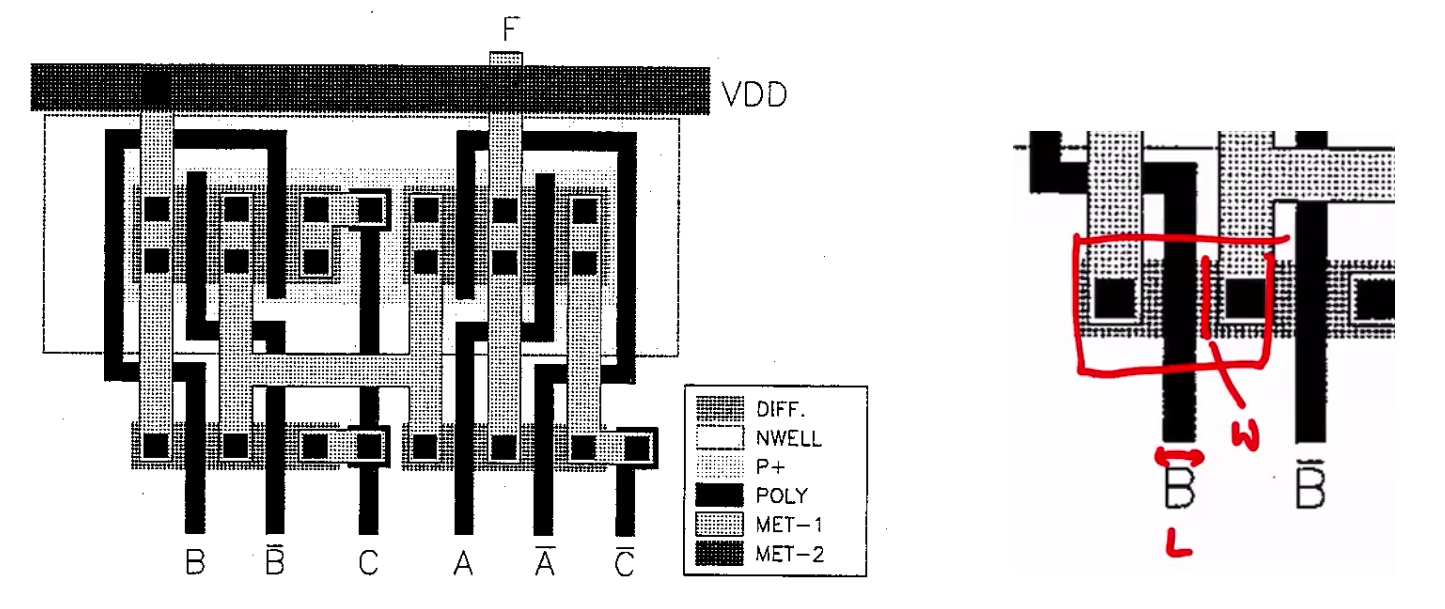
\includegraphics[width=0.75\linewidth]{img/transistore_circ_intergatas.png}
    \caption{Il circuito integrato della funzione (1999)}
    
\end{figure}

Per gli attuali circuiti è normale avere 6/8 livelli di metallizzazione, semplifica molto il passaggio delle piste.

\newpage
\section{Considerazioni}

La	logica a	pass	transistor	o	a	transmission gate	è non	\textbf{restoring}: tutto il rumore lo	ritroviamo in	uscita, per eliminare il rumore basta mettere un inverter in uscita.

La	logica CMOS	ripulisce invece il segnale a	causa dei margini di	rumore, dunque la	soluzione è quella di	introdurre dei buffer	CMOS	 regolarmente lungo il cammino logico in	modo da	ripristinare i livelli.


\paragraph{Errore da non fare 1: }

Evita di lasciare l'uscita flottante, deve esserci sempre uno ed un solo percorso (altrimenti non sappiamo dove vada l'uscita) da ingresso ad uscita.


\paragraph{Errore da non fare 2:}
La	logica a	pass	transistor	non	porta	l'uscita alla tensione di	alimentazione. Anche in	questo caso si utilizza un	buffer	o	un	inverter	in	serie al	segnale. Si	perdono però un	po'	i vantaggi della riduzione di	area. 

Poiché il segnale è degradato,	attenzione a	non	pilotare il gate di	un	altro pass,	o	si perde una ulteriore tensione di	soglia! Quindi si perde una tensione di soglia ogni volta che si passa da GS.


\begin{figure}[htbp]
    \centering
    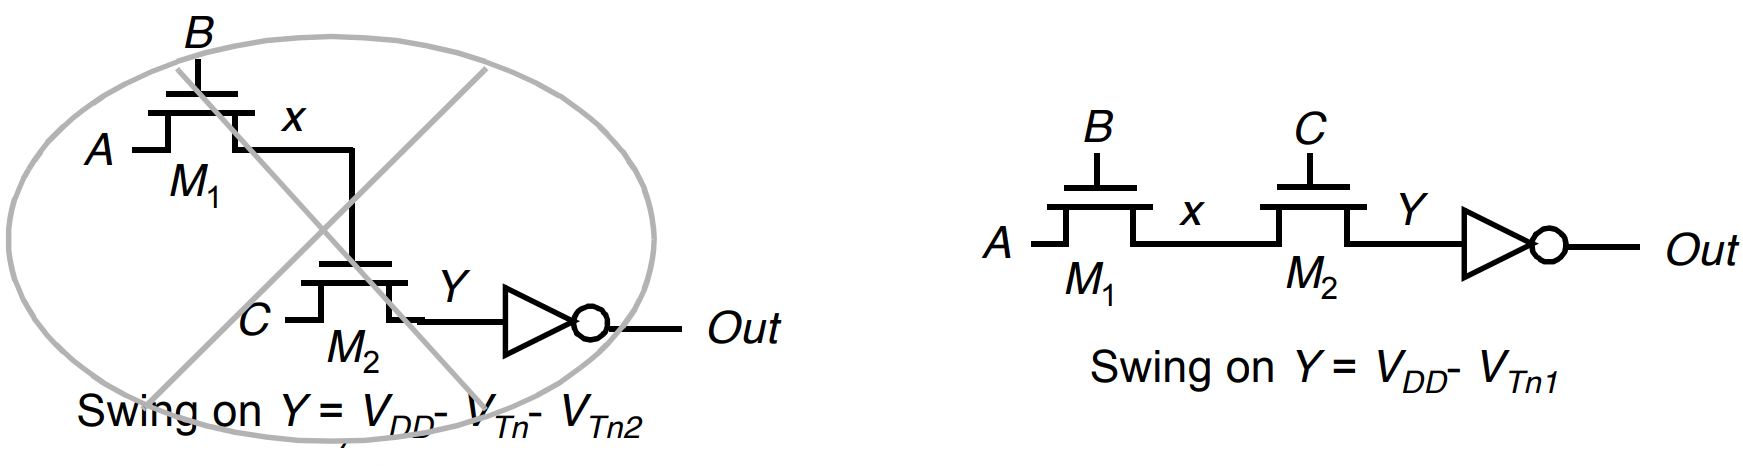
\includegraphics[width=0.75\linewidth]{img/non_fare.png}  
    
\end{figure}

Nell'immagine più a destra invece non si perdono due tensioni di soglia, bensì solamente una.
